
\documentclass[]{aiaa-tc}% insert '[draft]' option to show overfull boxes

\usepackage{amsmath}
 \usepackage{varioref}%  smart page, figure, table, and equation referencing
 \usepackage{wrapfig}%   wrap figures/tables in text (i.e., Di Vinci style)
 \usepackage{threeparttable}% tables with footnotes
 \usepackage{dcolumn}%   decimal-aligned tabular math columns
  \newcolumntype{d}{D{.}{.}{-1}}
 \usepackage{nomencl}%   nomenclature generation via makeindex
  \makenomenclature
 \usepackage{subfigure}% subcaptions for subfigures
 \usepackage{subfigmat}% matrices of similar subfigures, aka small mulitples
 \usepackage{fancyvrb}%  extended verbatim environments
  \fvset{fontsize=\footnotesize,xleftmargin=2em}
 \usepackage{lettrine}%  dropped capital letter at beginning of paragraph
 \usepackage[dvips]{dropping}% alternative dropped capital package
 \usepackage[colorlinks,filecolor=black,citecolor=black,linkcolor=black]{hyperref}%  hyperlinks [must be loaded after dropping]
 \usepackage{graphicx}
 \usepackage[section]{placeins}
 \usepackage{tikz}
 \usepackage{threeparttable}
%\usepackage{ltxtable}
\usepackage{multicol}
\usepackage{float}
\usepackage{gensymb}
\usepackage{minted}

 
\usepackage[nocomma]{optidef}
\usepackage{color, colortbl}
\definecolor{Gray}{gray}{0.9}
\definecolor{LightCyan}{rgb}{0.88,1,1}

% \usepackage[printwatermark]{xwatermark}
% % \newwatermark*[allpages,opactiy=0.3,color=red!50,angle=45,scale=3,xpos=0,ypos=0]{DRAFT}
% \newsavebox\mybox
% \savebox\mybox{\tikz[color=red,opacity=0.15]\node{DRAFT};}
% \newwatermark*[allpages, angle=45, scale=10, xpos=-20,ypos=15]{\usebox\mybox}

\setlength{\belowcaptionskip}{-5pt}
\setlength{\abovecaptionskip}{-5pt}

% \usepackage{draftwatermark}
% \SetWatermarkText{Draft}
% \SetWatermarkScale{8}

% Allow align to span pages
\allowdisplaybreaks

 \title{X-57 Mod 2 Motor Thermal Analysis}

 \author{
  Jeffrey C. Chin,\thanks{Propulsion Systems Analysis Branch, jeffrey.c.chin@nasa.gov, AIAA Member.} \
  Thomas T. Tallerico, \thanks{Rotating Systems Branch, thomas.t.tallerico@nasa.gov, AIAA Member.} \
  and Andrew D. Smith, \thanks{Aerospace Engineer, Vantage Partners LLC, Brookpark OH, andrew.d.smith-1@nasa.gov AIAA Member.} \\
  {\normalsize \itshape NASA Glenn Research Center, Cleveland, OH, 44135, U.S.A.} }

 % Data used by 'handcarry' option
 \AIAApapernumber{2017}
 \AIAAconference{AIAA Aviation, June 5-9, Atlanta GA}
 \AIAAcopyright{\AIAAcopyrightD{YEAR}}

 % Define commands to assure consistent treatment throughout document
 \newcommand{\eqnref}[1]{(\ref{#1})}
 \newcommand{\class}[1]{\texttt{#1}}
 \newcommand{\package}[1]{\texttt{#1}}
 \newcommand{\file}[1]{\texttt{#1}}
 \newcommand{\BibTeX}{\textsc{Bib}\TeX}
 
 % Change the spacing before/after equations
 \expandafter\def\expandafter\normalsize\expandafter{%
    \normalsize
    %\setlength\abovedisplayskip{10pt}
    \setlength\belowdisplayskip{20pt}
    %\setlength\abovedisplayshortskip{10pt}
    \setlength\belowdisplayshortskip{20pt}
}

 % Spacing between equations
\setlength{\jot}{10pt}

\begin{document}

\maketitle

\begin{abstract}

This work covers the refinement of thermal models from design estimates to actual fabricated performance. Matching the experimental data of the first fully electrified version of the X-57 Maxwell experimental vehicle requires high fidelity thermal analysis to sufficiently capture the electric motor and inverter temperature profiles. Qualification test data of the motors and inverters is used to validate finite element analysis models, which are then used to predict thermal performance over various notional mission transients. An additional thermal-hydraulic models is used to estimate flow characteristics through the propulsor nacelle and component heat sinks. After calibration of the higher order models, overall component sizing and peak temperature constraints can be distilled to reduced order models, to improve model flexibility and utility. The methods and experiments described are a snapshot of on-going work and include challenges encountered during motor performance verification.



\end{abstract}

%\printnomenclature% creates nomenclature section produced by MakeIndex

%\include{Nomenclature}
\section{Nomenclature}

\begin{multicols}{2}
 \begin{tabbing}
  XXXXXX \= XXXXXXXXXXXXXXXXXXXXXXXXXXXXXXXXXXXX \= \kill % first line sets tab stop
  %Term \> Description \> Units \\
  
  %$A$ \> cross sectional Area $(m^{2})$ \\
  $B$ \> peak magnetic field flux density $(\frac{Nm}{A})$\\
  $\Delta B$ \> peak to peak flux density $(\frac{Nm}{A})$\\
  $C_f$ \> skin friction coefficient $(-)$\\
  $C_p$ \> specific heat $(\frac{J}{K})$\\
  $Cu_F$ \> copper Fill Factor $(-)$\\
  $Dh$ \> hydraulic diameter $(m)$\\
  %$\epsilon$ \> emissivity \\
  $F$ \> force $(N)$\\
  $f$ \> friction factor $(-)$\\
  $f_e$ \> electrical frequency $(Hz)$\\
  $g$ \> gravity $(\frac{m^{2}}{s})$\\
  $HC$ \> heat capacity $(\frac{J}{K})$\\
  $h$ \> convection heat transfer coefficient $(\frac{W}{m^{2}K})$ \\
  $I$ \> supply current $(A)$\\
  $\eta$ \> efficiency $(-)$\\
  $I$ \> current $(A)$\\
  $k$ \> thermal conductivity$(\frac{W}{m*K})$\\
  $l$ \> length $(m)$\\
  $m$ \> mass $(kg)$\\
  %$M_{chord}$ \> Standard mean chord $(m)$\\
  $Nu$ \> Nusselt number $(-)$\\
  $n_p$ \> number of parallel paths $(-)$\\
  $P$ \> power $(W)$ \\
  \\
  \\
  $P_{r}$ \> Prandtl Number $(-)$\\
  $\dot{Q}$ \> heat transfer rate $(\frac{W}{s})$ \\
  $R$ \> electrical resistance $(\Omega)$\\
  $Ra_D$ \> Rayleigh Number $(-)$\\
  $R_{e}$ \> Reynolds Number $(-)$\\
  $T$ \> temperature $(K)$\\
  $t$ \> time $(s)$\\
  $V$ \> velocity $(\frac{m}{s})$\\
  $\alpha$ \> thermal diffusivity $(\frac{m^{2}}{s})$\\
  $\delta$ \> air-gap distance $(m)$\\
  $\gamma_a$ \> atmospheric ratio of specific heats $(-)$\\
  %$q'$ \> heat transfer rate per unit length $(\frac{W}{m*s})$\\
  $\nu$ \> kinematic viscosity $(\frac{m^2}{s})$\\
  $\mu$ \> dynamic viscosity $(mPa*s)$\\
  $\mu_f$ \> coefficient of friction $(-)$\\
  $\rho$ \> density $(\frac{kg}{m^{3}})$\\
  $\rho$ \> material resistivity $(\ohm*m)$\\
  $\phi$ \> phase offset $(rad)$\\
  %$\rho_{r}$ \> hemispherical reflectivity\\
  %$S_{wing}$ \> Wing Area $(m^{2})$ \\
  %$\sigma$ \> Stefan-Boltzmann Constant $(\frac{W*m}{K^{4}})$ \\
  $\tau$ \> torque $(N*m)$\\
  $\theta$ \> angle integration constant $(rad)$\\
  %$u_{o}$ \> free stream velocity $(\frac{m}{s})$\\
  $\nu$ \> kinematic viscosity of air $(\frac{m^{2}}{s})$\\
  $\omega$ \> angular velocity $(\frac{rad}{s})$\\

 \end{tabbing}
\end{multicols}
\newpage

\nomenclature{\beta}{test}

\section{Introduction}

The NASA X-57 experimental aircraft aims to demonstrate all-electric flight, specifically using distributed electric propulsion to achieve 4.8x better efficiency at cruise. The development is segmented into 4 distinct vehicle configurations, referred to as ``mods'' as shown in Figure \ref{fig:Mod2Big}. Mod 2, shown on the left, uses a modified Tecnam P2006T fuselage and wing, with the inboard propellers powered by electric motors and batteries. After successful flight in this configuration, the propellors are moved to the wingtips, and the wing area is reduced by a factor of 2.5 using high-aspect area wings in Mod 3. The final Mod 4 configuration implements six small high lift motors along each wing to provide additional lift during climb and final approach, while being folded conformal to the nacelle during cruise. This progression is shown in the right column of Figure \ref{fig:Mod2Big}. \cite{falck_X57}
\cite{Borer_2016}

This work covers the refinement of thermal models from design estimates to actual fabricated performance. The motor and inverters were manufactured by Joby motors and have been ground tested at NASA Armstrong. Testing was performed on the AirVolt test stand as part of qualification testing, with the secondary intent of verifying thermal models. To further validate efficiency estimates, the motors are undergoing further testing on a dynamo-meter in a more controlled thermal environment. This paper captures the work, results and lessons learned to-date.

\begin{figure}[!htb]% order of placement preference: here, top, bottom
	\centering
	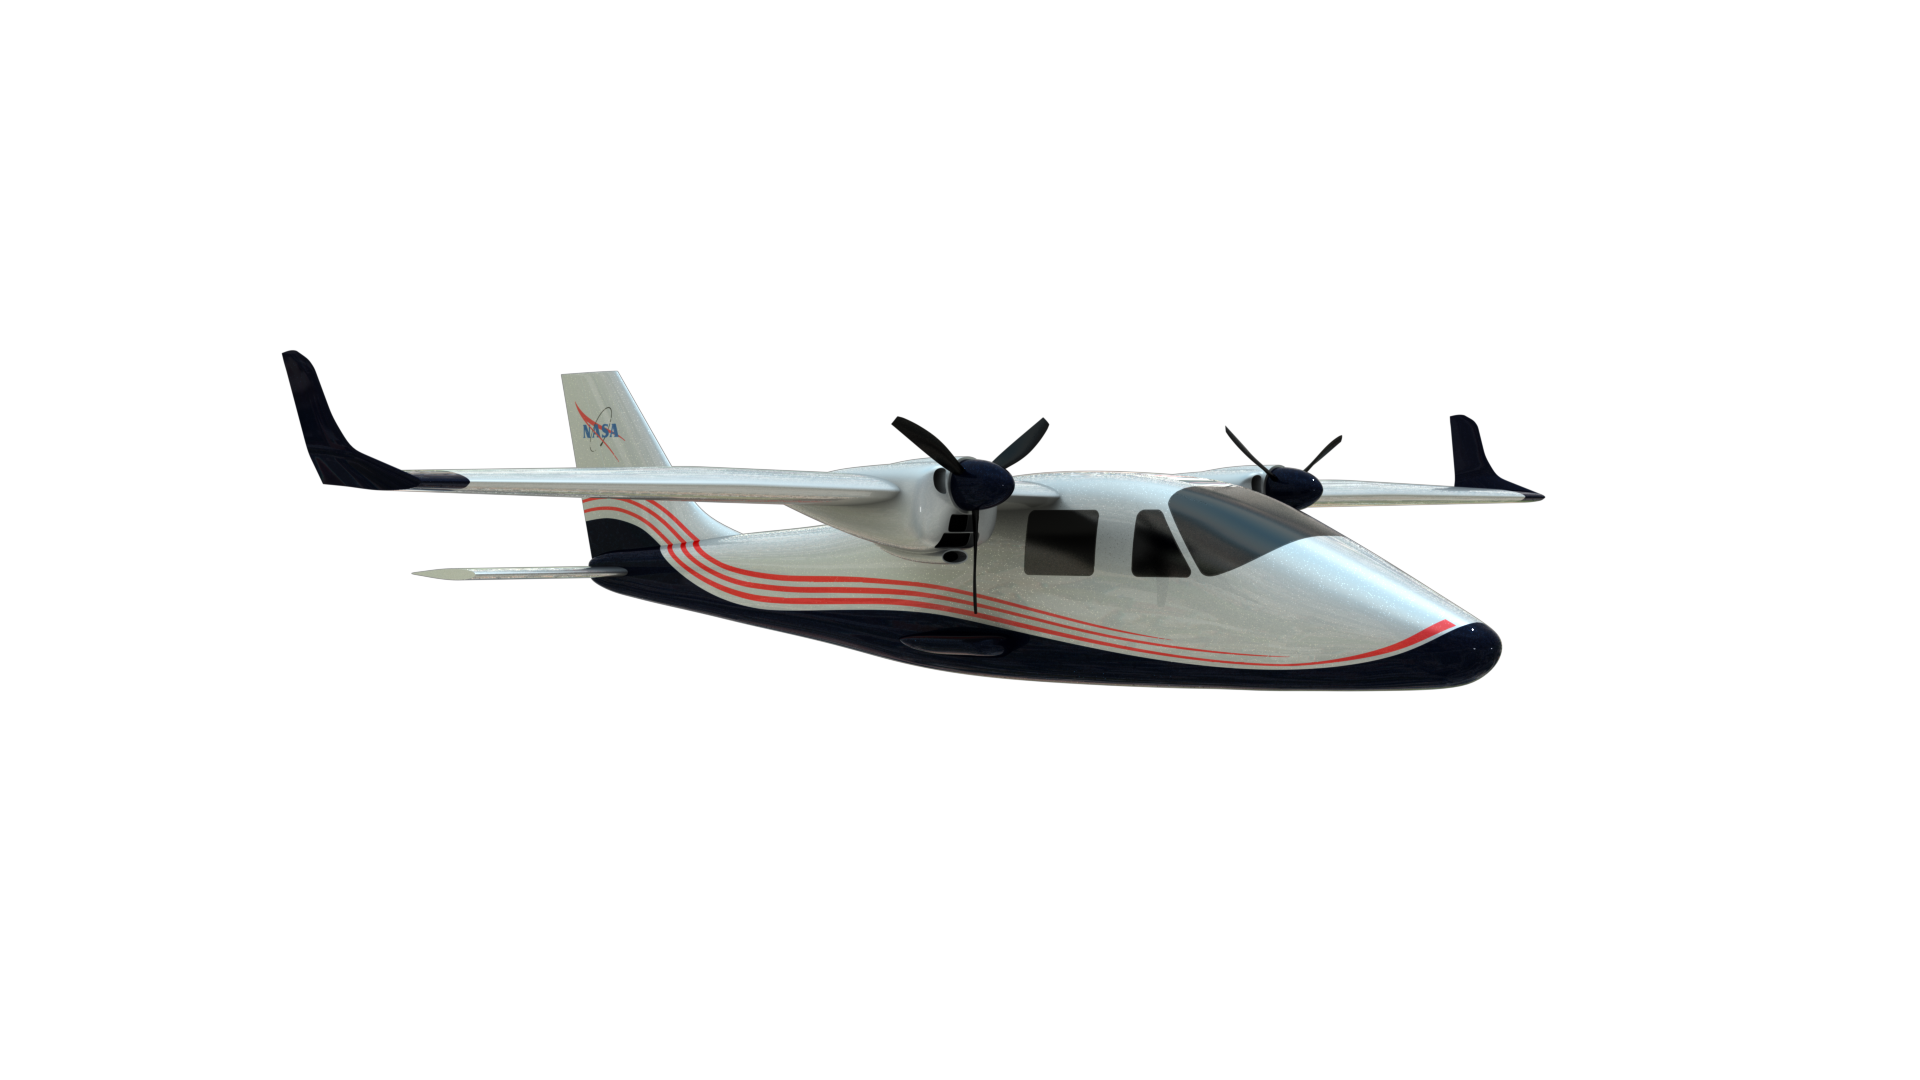
\includegraphics[width=0.75\textwidth]{figures/X57_mod2.png}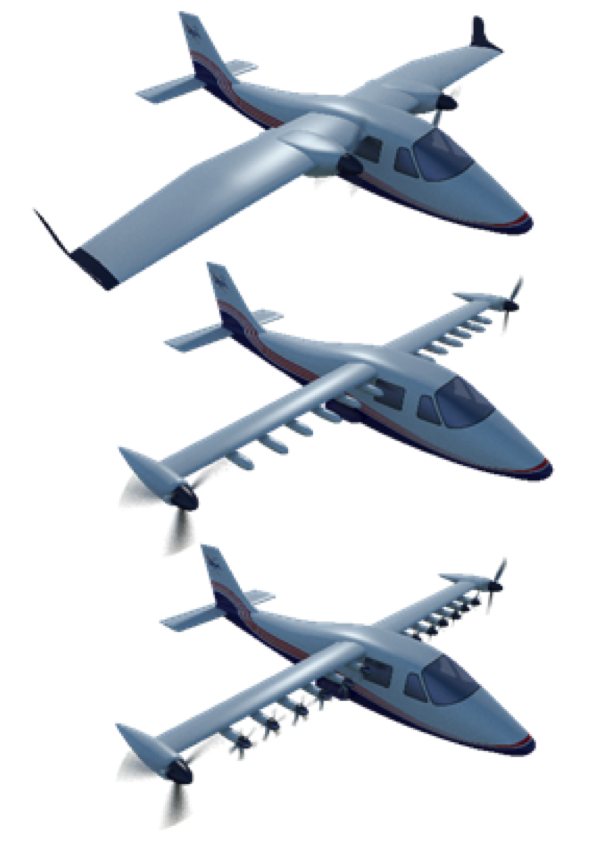
\includegraphics[width=0.25\textwidth]{figures/Mod234.png}
	\caption{NASA's X-57 "Maxwell" Aircraft, (Left) Mod \#2 Variant, (Right) Evolution of Mod \#2, 3, \& 4 Variants}
	\label{fig:Mod2Big}
\end{figure}

% \begin{figure}[!htb]% order of placement preference: here, top, bottom
% 	\centering
%     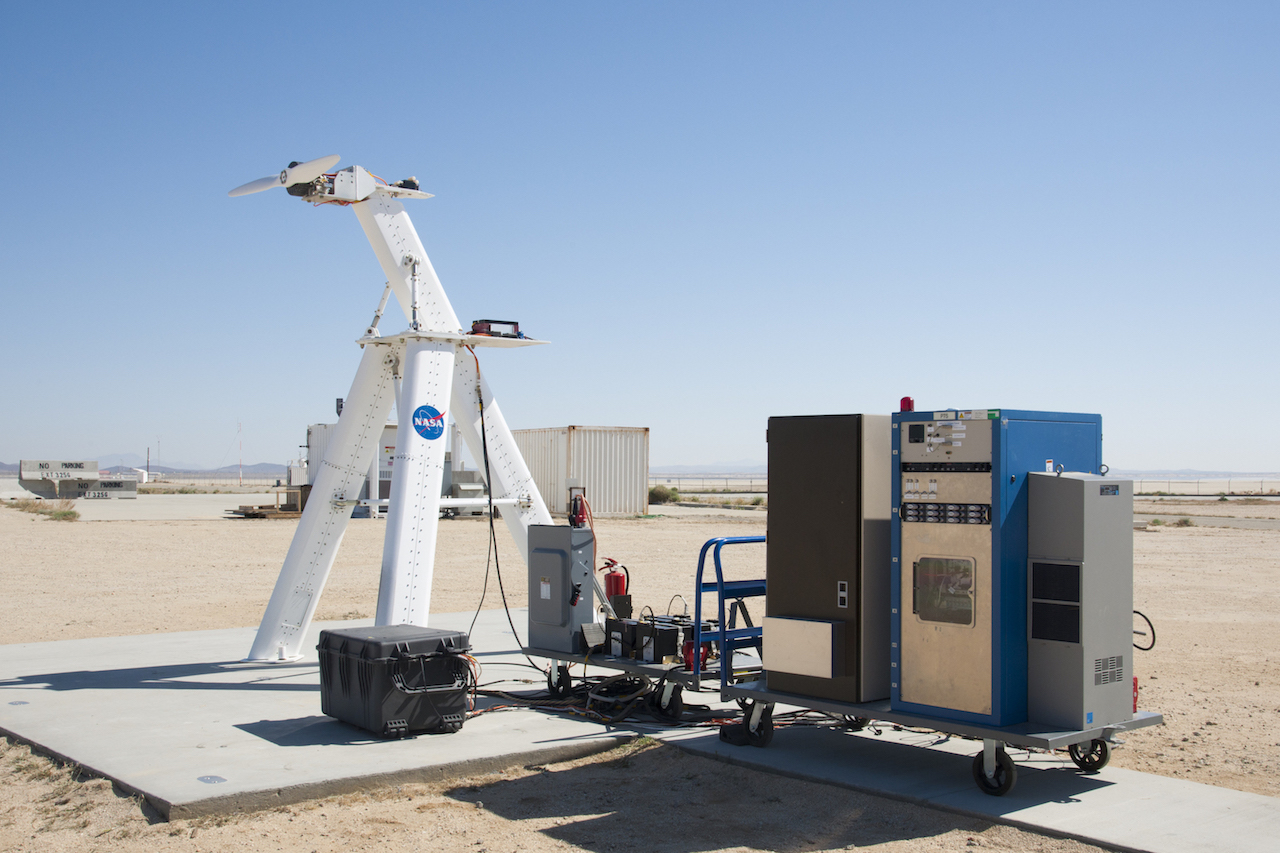
\includegraphics[width=0.5\textwidth]{figures/airvoltOld.jpg}
% 	\caption{(Left) AirVolt JM-X57 motor installed without spinner, with positioned cooling cart yellow tubing (Right) Original stand prior to JM-X57 testing}
% 	\label{fig:airvolt}
% \end{figure}

\subsection{Experimental Setup}
\subsubsection{AirVolt Test Stand and Experimental Setup}

AirVolt is an open-air test stand located at NASA's Armstrong Flight Research Center designed for testing electric motors and controllers.\cite{Aamod_2015} \cite{Papathakis}A profile and aft shot can be seen in Figure \ref{fig:airvolt2}. In preparation for X-57's first flight, the cruise motors are subjected to endurance and vibration testing per FAR Part 33 Airworthiness Standards. The stand measures torque, thrust, voltage, current, power, acceleration, and temperature. Initial full power tests were run for a duration of five minutes, with 16 thermistor locations on the motor. Due to a maximum allowable temperature of 100 degrees C, portable cooling carts were used to blow up to 600 lbs/min of 8 \degree C air directly onto the propeller spinner.  The test discussed in this paper had three cooling carts active, with a commanded torque of 255 N-m at 2250 rotations per minute to simulate a 60kW full power climb. Each run started at a 27\degree C winding temperature and terminated at 100\degree C. The first run lasted 21:06 minutes. The three full throttle commands lasted 6:53, 6:37, 4:28 minutes respectively and are plotted in Figure \ref{fig:airvoltData}

\begin{figure}[!htb]% order of placement preference: here, top, bottom
	\centering
	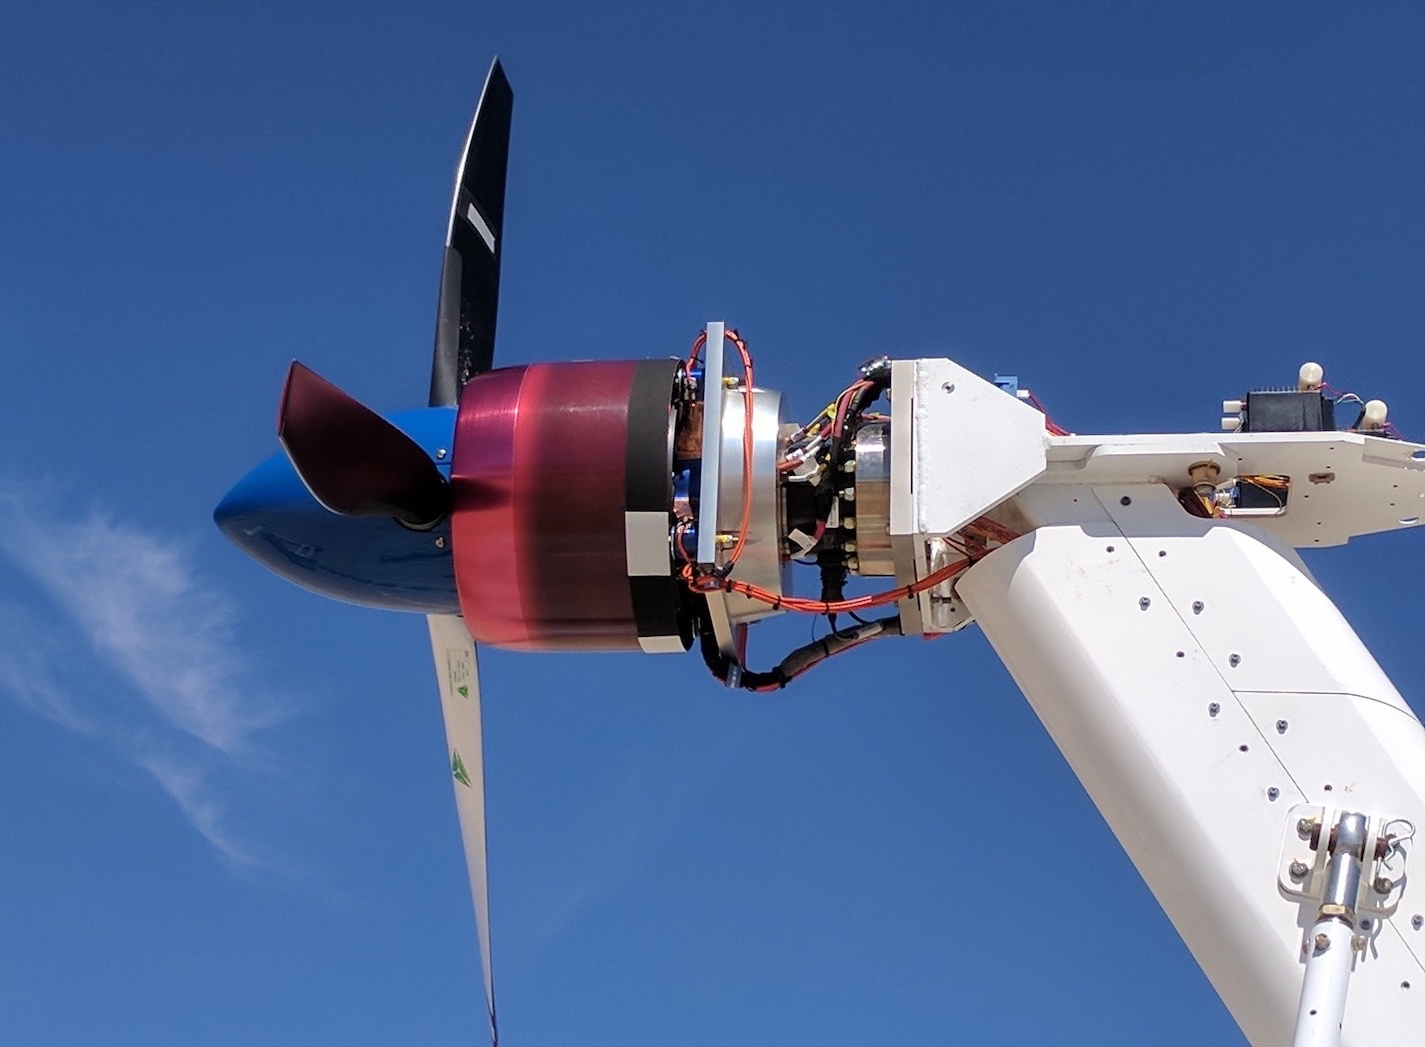
\includegraphics[width=0.5\textwidth]{figures/AirVoltSide.jpg}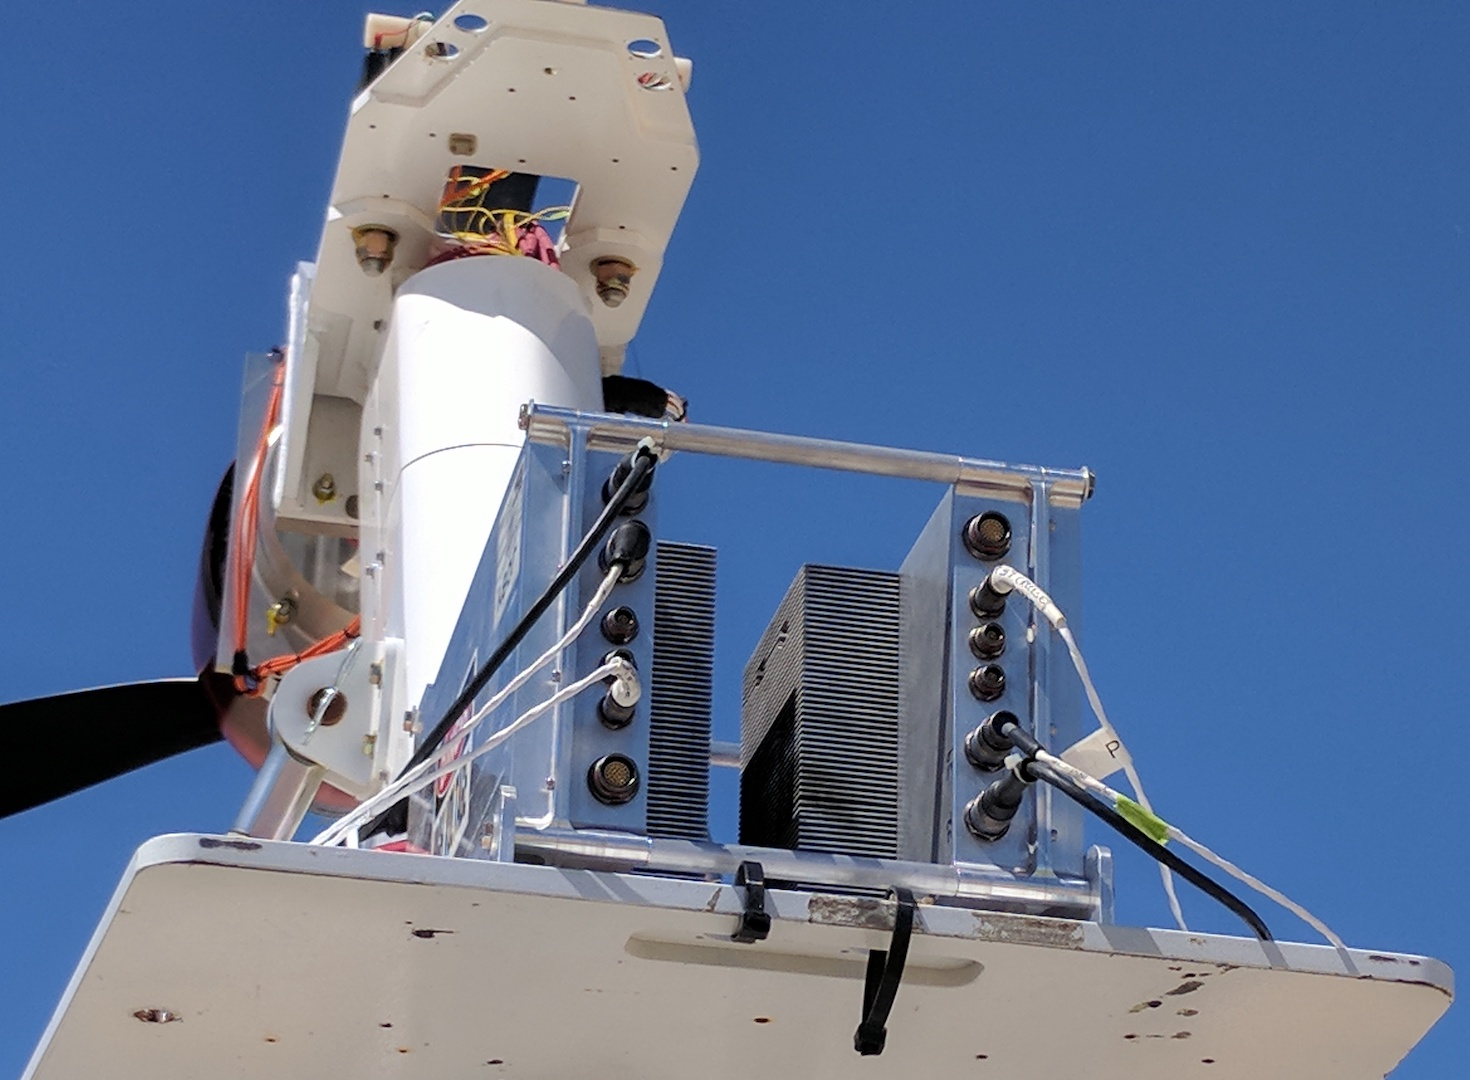
\includegraphics[width=0.5\textwidth]{figures/AirVolt_Back.jpg}
	\caption{(Left) Close up of the JM-X57 motor and thrust mount. (Right) Back-to-Back Inverters}
	\label{fig:airvolt2}
\end{figure}

\begin{figure}[!htb]% order of placement preference: here, top, bottom
	\centering
	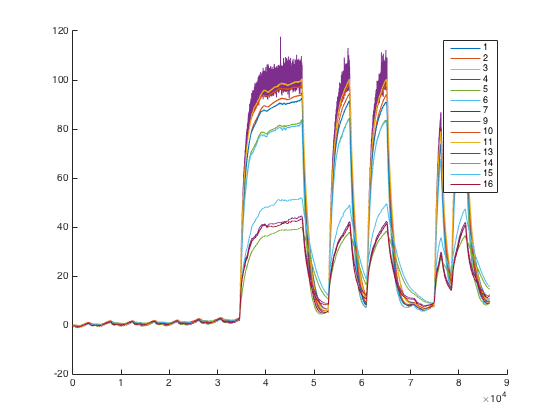
\includegraphics[width=0.75\textwidth]{figures/AirvoltMotor.png}
	%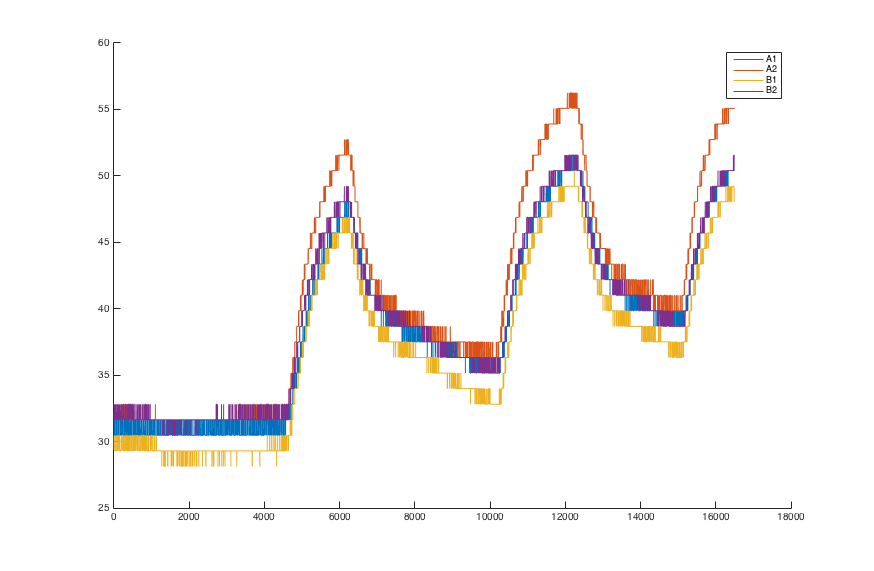
\includegraphics[width=0.5\textwidth]{figures/AirvoltCMC.png}
	\caption{(Left) Airvolt test run motor thermocouple reading (Right) Inverter chip temperature reading.
    10/12 9:29am Test 1 60kW, 3 cooling carts, airspeed unknown, steady-state reached (almost).}
	\label{fig:airvoltData}
\end{figure}

\subsubsection{Motor Sensor Installation}
A negative temperature coefficient (NTC) thermistor was installed every fourth coil during the motor manufacturing process. The sensors were inserted between the coils and stator yolk at the most radially inward accessible location of the slot. The sensors were installed after the teeth laminations were assembled but before motor winding. Unfortunately in hindsight, this resulted in inconsistent readings as some sensors were influenced more by the steel than the coil windings. After coiling, the stator windings were potted with a low viscosity wicking epoxy. The intended purpose of this epoxy is to secure the windings against movement and vibration, and to provide a good thermal path to the steel laminations. However, the slot is intentionally not entirely filled to save mass. This further exacerbates the variability in the NTC sensor thermal mounting depending on the level of thermal contact.

The following sections summarize of the relevant thermal results obtained. Efficiency of the controllers and motors are surmised based on operating voltage, current, and temperature rise of the system. Heat generation in the motor is split between various parts of the stator and rotor, so the percentage of heat through each component must be estimated. Additional confounding factors including ambient cooling, and spinner induced flow must also be considered. To determine efficiency, a high-fidelity COMSOL model of the motor was created to determine the temperature distribution within each subcomponent and calibrated against multiple installed thermocouple locations. A transient execution is performed then calibrated against test data to compensate for uncontrolled cooling.


\subsubsection{Data Analysis}

Test data on Airvolt was sampled at 60 samples per second, however the provided raw thermistor data was not calibrated, since it was not the main focus of the trial run. Therefore, each sensor values were individually offset to the mean temperature reading before the motor was run. A large spread in peak temperature was recorded across various winding positions, so the peak model temperature was calibrated against the peak recorded thermistor reading. Temperature readings drastically below the peak reading were assumed to have poor thermal contact with the windings. The highest temperature reading also appeared to have substantial EMI noise, so the data was smoothed via a Fast Fourier Transform (FFT) in Matlab.

\setminted{fontsize=\small,baselinestretch=1}
\begin{minted}{matlab}
alpha = 0.1; % tune-able parameter 
data(2:n-1) = alpha*data(2:n-1) + (1-alpha)*0.5*(data(1:n-2)+data(3:n)) % clip symmetrically
f = fft(data) % take Fast Fourier Transform
f(n/2+1-20:n/2+20) = zeros(40,1); % remove high frequency content
smoothed_data = real(ifft(f)) % revert back to time domain, ignore small complex noise
\end{minted}

In this implementation, alpha is a tune-able parameter, with the 20 highest frequencies cut out symmetrically. Only the real component of the inverse FFT is copied, since any imaginary component only exists due to rounding precision.

The subsequent analysis focuses on matching models to the first transient shown in Figure \ref{fig:airvoltData}. Since it was the first run, the entire motor starts evenly at ambient conditions, and the full power operation was sustained long enough to approximately reach a steady-state.

\section{Thermal Modeling}

\subsection{Finite Element Thermal Model}

Power lost to motor inefficiencies manifests as heat in the rotor, stator, and bearings. By tracking the transient temperature across a run, the overall motor efficiency can be estimated. To quantify the total heat loss of the system based on temperature, there must be a detailed accounting of all of the thermal properties, resistances, and cooling sources within the system. A Finite Element Analysis (FEA) thermal model was built in COMSOL to calculate the heat distribution in the motor stator. To improve simulation speed, an axi-symmetric cut of the stator was simulated, assuming the heating would be roughly symmetrical for every wedge. The thermal losses in the rotor were not experimentally measured, and therefore were not considered in this portion of the model. These rotor losses, due to the eddy currents and mechanical friction, are considered in subsequent sections. A particular 30 degree slice of the stator was chosen to maintain the relevant structural members. The model includes the main aluminum support trusses and heat sink fins, iron stator laminations, copper windings, and Nomex slot liners. Two separate models scenarios were run to match against two unknowns in the experimental data. First a steady-state run matching the end conditions of the first full power pulse; this model could be simulated quickly to evaluate the model sensitivity to various parameters. The second model was driven transiently to match the power profile of the AirVolt tests, and thermal convection terms across an array of time points. Between these to scenarios, loss and heat convection terms were calibrated until the temperature profiles matched.

The first challenge was estimating the overal heat transfer coefficient of the heat sink, given uncertainty in the cooling cart air velocity.
$3,000<Re<10,000$

\begin{equation}
Dh = \frac{2*a*b}{a+b} = 0.00358,
a = 0.002, b = 0.017, l = 0.105
\label{eq:Dh}
\end{equation}

\begin{equation}
Re = \frac{V*Dh*\rho}{\nu}
\label{eq:Re}
\end{equation}

\begin{equation}
Pr = \frac{\nu*Cp}{k}
\label{eq:Pr}
\end{equation}

\begin{equation}
Nu_{devel} = \frac{\frac{f}{8}*(Re-1000)*Pr}{1+12.7*\frac{f}{8}^{0.5}*(Pr^{\frac{2}{3}}-1)}
\label{eq:Nu}
\end{equation}

\begin{equation}
h = \frac{Nu*k}{Dh}
\label{eq:h}
\end{equation}

\begin{equation}
ROC_{T} = \frac{\delta T}{\delta t} = \frac{q'_{stator}-q'_{out}}{HC}
\label{eq:ROC}
\end{equation}

\begin{table}[hbt!]
\caption{\label{tab:COMSOL} Model Assumptions}
\centering
\begin{tabular}{lcccc}
Material  & $\rho$ $\frac{J}{kg*K}$ & $Cp$ $\frac{J}{kg*K}$  & $K_{radial}$ $\frac{W}{m*K}$ & $K_{axial}$ $\frac{W}{m*K}$\\\hline
JNEX900 Steel & 7650& 500& 20& 20\\
Aluminum 6063-T83   & 2700  & 900 & 201& 201  \\
Copper & 8960 & 385 & 400& 400\\
Epoxy & 1225 & 1000 & 1& 1 \\
Copper Epoxy Bulk & 4705.75 & 723.25 & 1.8145 & 180.55\\
Slot Liner (.25mm thick) &-&-&139 & 139\\\hline
\end{tabular}
\end{table}

\begin{equation}
K_{radial} = \frac{ke*kc}{(1-CuF)*kc + CuF*k3}
\label{eq:kradial}
\end{equation}

\begin{equation}
K_{axial} = CuF*kc + (1-CuF)*ke
\label{eq:kaxial}
\end{equation}

\begin{figure}[!htb]% order of placement preference: here, top, bottom
	\centering
	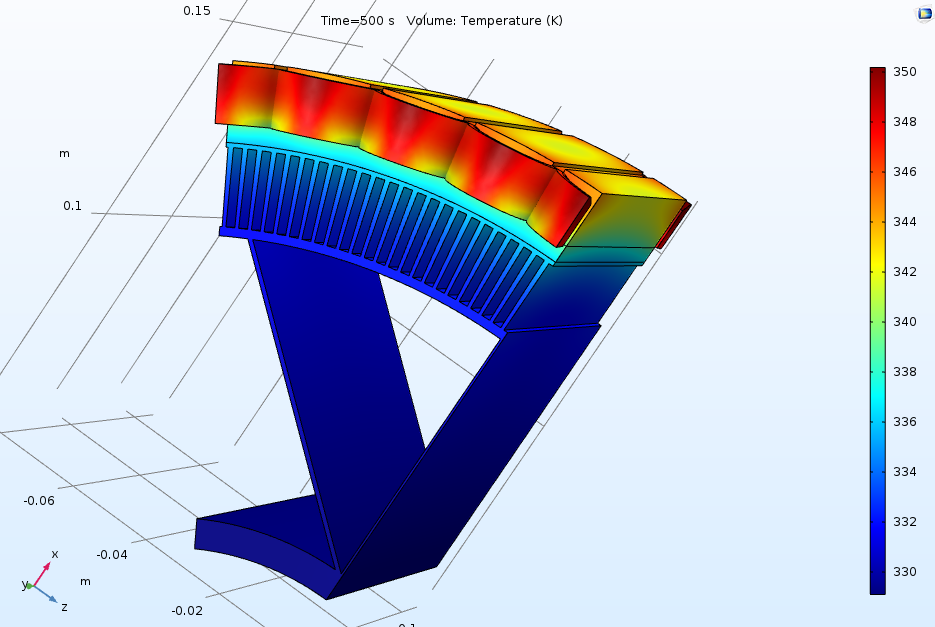
\includegraphics[width=0.75\textwidth]{figures/jmx57_motor_comsol.png}
	\caption{COMSOL}
	\label{fig:comsol}
\end{figure}

Using a steady-state model a range of airspeeds and motor efficiencies are run in a design of experiments. To improve simulation speed, the model is further simplified to a 2D slice of the stator at the center of the coil. A polynomial is then fit through all the cases where the steady state is 100C to determine a trend-line of losses based on airspeed.
Next a transient model is run for three different points from the trend-line calculated, this data is then compared against a separate AirVolt test that didn't have any active air cooling. The transient test was compared to the uncooled test data since it was closer to adiabatic temperature rise, without cooling airflow as an additional confounding factor. Based on the three computed heat rise rates, a specific airspeed and loss combination will match the temperature rise per time $(\frac{dT}{dt})$ of the experimental data.

\begin{figure}[!h]% order of placement preference: here, top, bottom
	\centering
	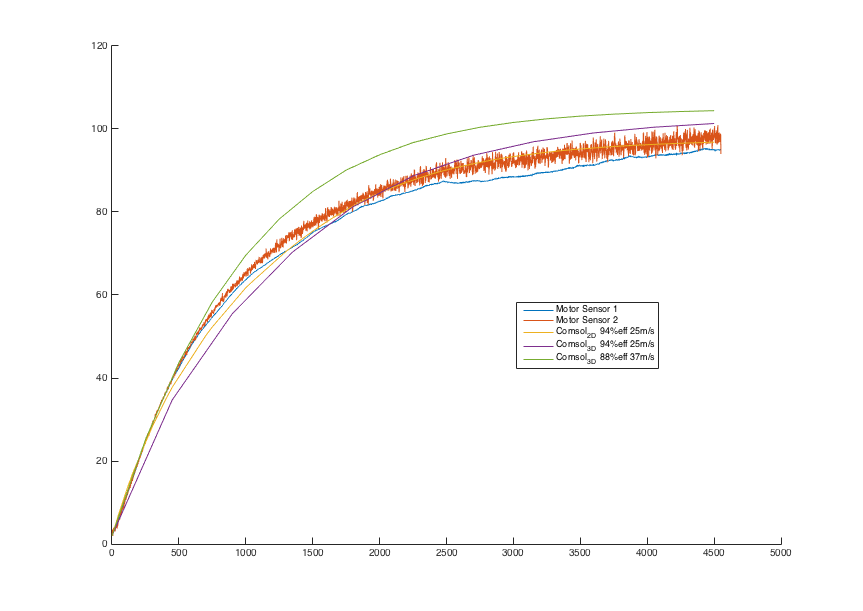
\includegraphics[width=1.0\textwidth]{figures/Temp_motor_1012_0929.png}
	\caption{}
	\label{fig:COMSOLresults}
\end{figure}

Figure \ref{fig:COMSOLresults} shows the results from various COMSOL model simulations compared to the experimentally recorded data. When using a 2D model, the data was best fit with a motor efficiency of 94\% and 25 $\frac{m}{s}$ cooling flow. Expanding the model back to a full 3D slice resulted in a noticeably higher heat capacity and final steady-state temperature. To match the initial temperature rise, the assumed motor losses had to be doubled, leading to an efficiency of 88\% instead of 94\%.

\subsubsection{Model Parameter Sensitivity}


\subsection{Thermal Hydraulic Flow Model}

The cruise propulsion system as installed in the Mod 2 vehicle consists of a single JMX57 motor driven by a pair of Cruise Motor Controller (CMCs).  The CMC location within the Mod 2 nacelle rules out the use of independent cooling air paths for the motor and controllers.  

\begin{figure}[!h]% order of placement preference: here, top, bottom
	\centering
	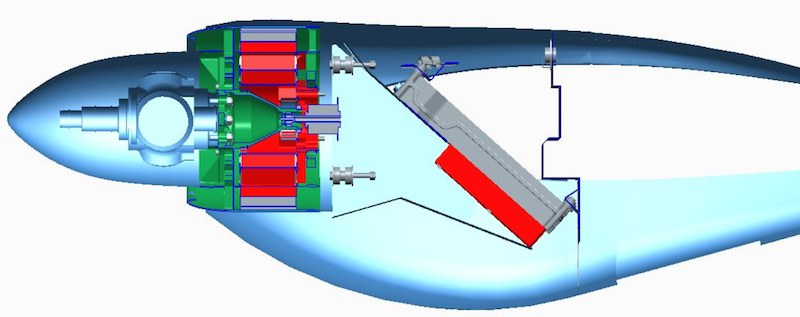
\includegraphics[width=1.0\textwidth]{figures/mod2_profile.png}
	\caption{Side profile view of the Mod2 cruise nacelle. Motor in green, heat sinks in red}
	\label{fig:Mod2Profile}
\end{figure}


Cruise motor cooling is achieved with a combined flow path (“cascaded” cooling) that passes sequentially both the motor and CMC fin rows.  The nacelle inlet is split into a pair of concentric annuli - the innermost directly supplies the JMX57 motor with cool air, while the outer annulus directly charges the nacelle interior volume.  Warm air exhausted by the motor mixes with the bypass air, and continues through the motor controller (CMC) duct before being vented overboard.  
This configuration differs from the proposed Mod 3 and Mod 4 cruise design with the inclusion of the bypass or “motor gap” inlet.  The proposed gap width is meant to provide clearance to the spinning outer diameter of the JMX57, an out-runner motor while still conforming to a nacelle outer mold line similar to the stock Tecnam p2006t aircraft. 
A concern raised during the evaluation of this ‘cascade’ cooling system (as applied to the Mod 2 nacelle) is the potential for air to bypass the JMX57 cooling fins in favor of the ‘gap’ inlet, resulting in a reduction in cooler performance for the highest power density component in the cruise assembly.  
To better understand the interaction between the design parameters of the Mod 2 nacelle flow path, a combined thermal-hydraulic model was created in CRTech Sinaps, a visual modeling tool for SINDA/FLUINT thermo-hydraulic networks. 

\begin{figure}[!htb]% order of placement preference: here, top, bottom
	\centering
	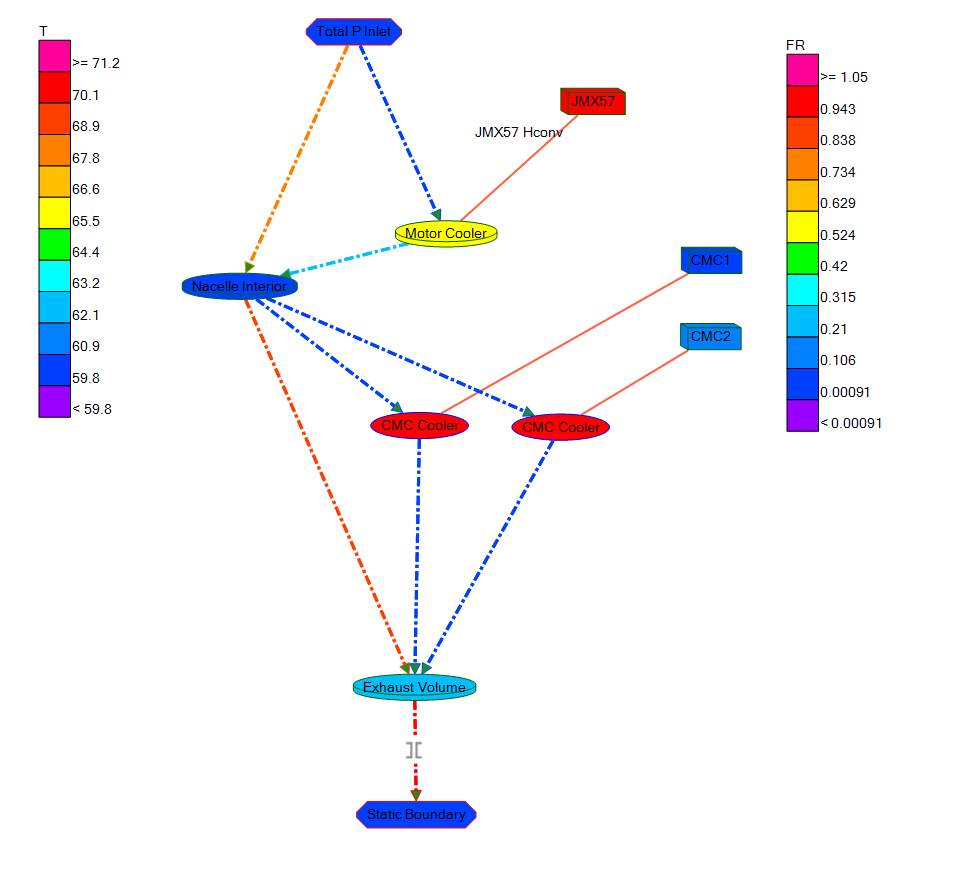
\includegraphics[width=0.75\textwidth]{figures/sinaps_paramsweep.PNG}
	\caption{Mod 2 Cruise Nacelle Flow Network in CRTech Sinaps}
	\label{fig:Sinaps}
\end{figure}

The flow network consists of boundary, plenum and connector fluid lumps.  Boundary lumps are defined by their respective static temperature and pressure, while plena are defined by their volume.  Fluid connections between lumps are defined by their length, hydraulic diameter, and flow area.  The steady state-flow is solved with a single-phase correlation model build into Sinda/FLUINT; a Darcy-Weisbach solution based a friction factor derived from a numerically smooth representation of the Moody Chart  (Darcy-Weisbach friction factor vs. Reynolds Number) \cite{CRtech_2013}.  A multiplication factor is used to represent multiple parallel, identical flow connectors (i.e. a parallel channel heat sink).  Specific flow connection parameters (hydraulic diameter, length, and area) were derived from CAD models provided of the Mod 2 nacelle, the JMX57 cooling fins, and an extruded fin profile selected for the CMC cooler.  

Each heat-dissipating component (JMX57 motor, CMC) was modeled using lumped parameters with a bulk specific heat (J/K) and thermal power dissipation.  The heat sources are coupled to the fluid network via forced convection ties.  Each tie is related to one or more fluid connectors to provide input parameters for the internal convection correlation appropriate for the flow solution.  A simple isothermal Nusselt number correlation (where Nu = 3.66) is used for low Reynolds number fluid paths, while turbulent convection coefficients are found via the Dittus-Boelter correlation. \cite{CRtech_2015}.  Transitional Reynolds number flows (2000 $<$ Re $<$ 4600) are modeled with Hausen’s transition correlation. \cite{Kays}


\subsection{Nacelle Gap Design Sweep}

Through testing, it was discovered that the motor heated up to it's maximum operational temperature faster than expected. Although the inverters did not experience high temperatures on the static test stand, the final configuration will expose the inverter heat sink to hot motor exhaust. This motivated a design study to determine the optimal spacing between the nacelle fairing and motor outer diameter to guarantee sufficient cooling for the inverters.

\begin{figure}[!htb]% order of placement preference: here, top, bottom
	\centering
	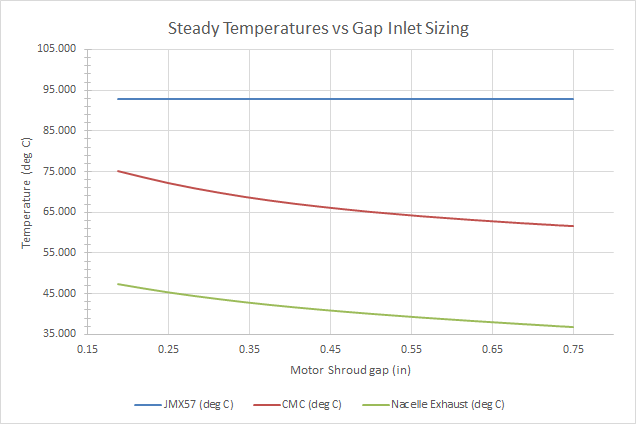
\includegraphics[width=.75\textwidth]{figures/gapsweep_results.png}
	\caption{Inverter Temperature Sensitivity to Fairing Gap Height}
	\label{fig:GapSweep}
\end{figure}

While the nacelle gap study is not predictive of actual component temperatures – as this requires higher fidelity conjugate heat transfer modeling.  Rather, the resulting steady lump temperatures are used to evaluate the overall cooling system performance sensitivity to the swept design parameters – specifically the “gap” inlet width.  Inlet conditions for the “gap inlet” study were chosen as a pessimistic  
A design sweep was conducted on the Mod 2 thermo-hydraulic network – focusing specifically on the sensitivity of motor and CMC operating temperatures to changes in the “gap” inlet size.  
The results of this sweep show little sensitivity in motor cooling performance to the size of the “gap” inlet – suggesting that the driving flow restriction in the network is downstream of the JMX57.  Of particular significance is the response of the CMC steady temperatures with increasing gap size:  increasing the volume of air that bypasses the motor results in lower operating temperatures for the CMCs without sacrificing motor cooling performance.  This effect diminishes past the nominal Mod 2 gap size of $\frac{3}{8}"$, but could be adapted to other X57 vehicle configurations (Mods 3 and 4) with little risk of compromising motor cooling. Further discussion of this gap sizing can be found in previous works. \cite{Schnulo}


\subsection{Two-dimensional performance and loss model}

The original motor design by Joby \cite{Dubois2016} estimated the efficiency of the motor for a range of rpms and torque settings as shown in figure \ref{fig:map}. This performance map is compared against a similar fidelity model developed in MotorSolve. Finally efficiency points from AirVolt testing provide a third comparison point showing achieved performance with uncertainty from measured quantities.

\begin{figure}[!htb]% order of placement preference: here, top, bottom
	\centering
	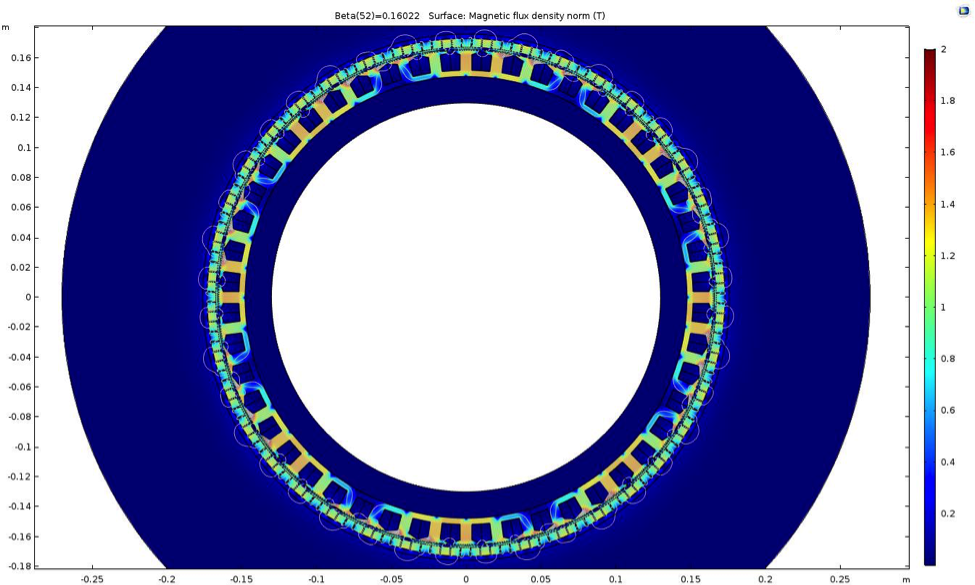
\includegraphics[width=1.0\textwidth]{figures/COMSOL_EM.png}
	\caption{}
	\label{fig:COMSOL_EM}
\end{figure}


A 2D FEA simulation of the motor was made using Comsol Multiphysics rotating machinery module in order to establish initial loss predictions. The FEA model was used to determine static torque vs current curves for the motor and the magnetic field in all components vs rotor position at nominal operating conditions. The magnetic field data was post processed to predict stator core loss, wire proximity loss, and eddy current loss in the magnets. Mechanical windage and bearing losses were also calculated. These losses were than used to scale the required torque and thereby the required current so that shaft power was maintain. Resistive losses were then predicted using this scaled up current. The models used for these loss calculations will be discussed in the following sections. An example result from the FEA model can be seen in Figure \ref{fig:COMSOL_EM}. Material properties used in this analysis are available in Table X.

\begin{figure}[!htb]% order of placement preference: here, top, bottom
	\centering
	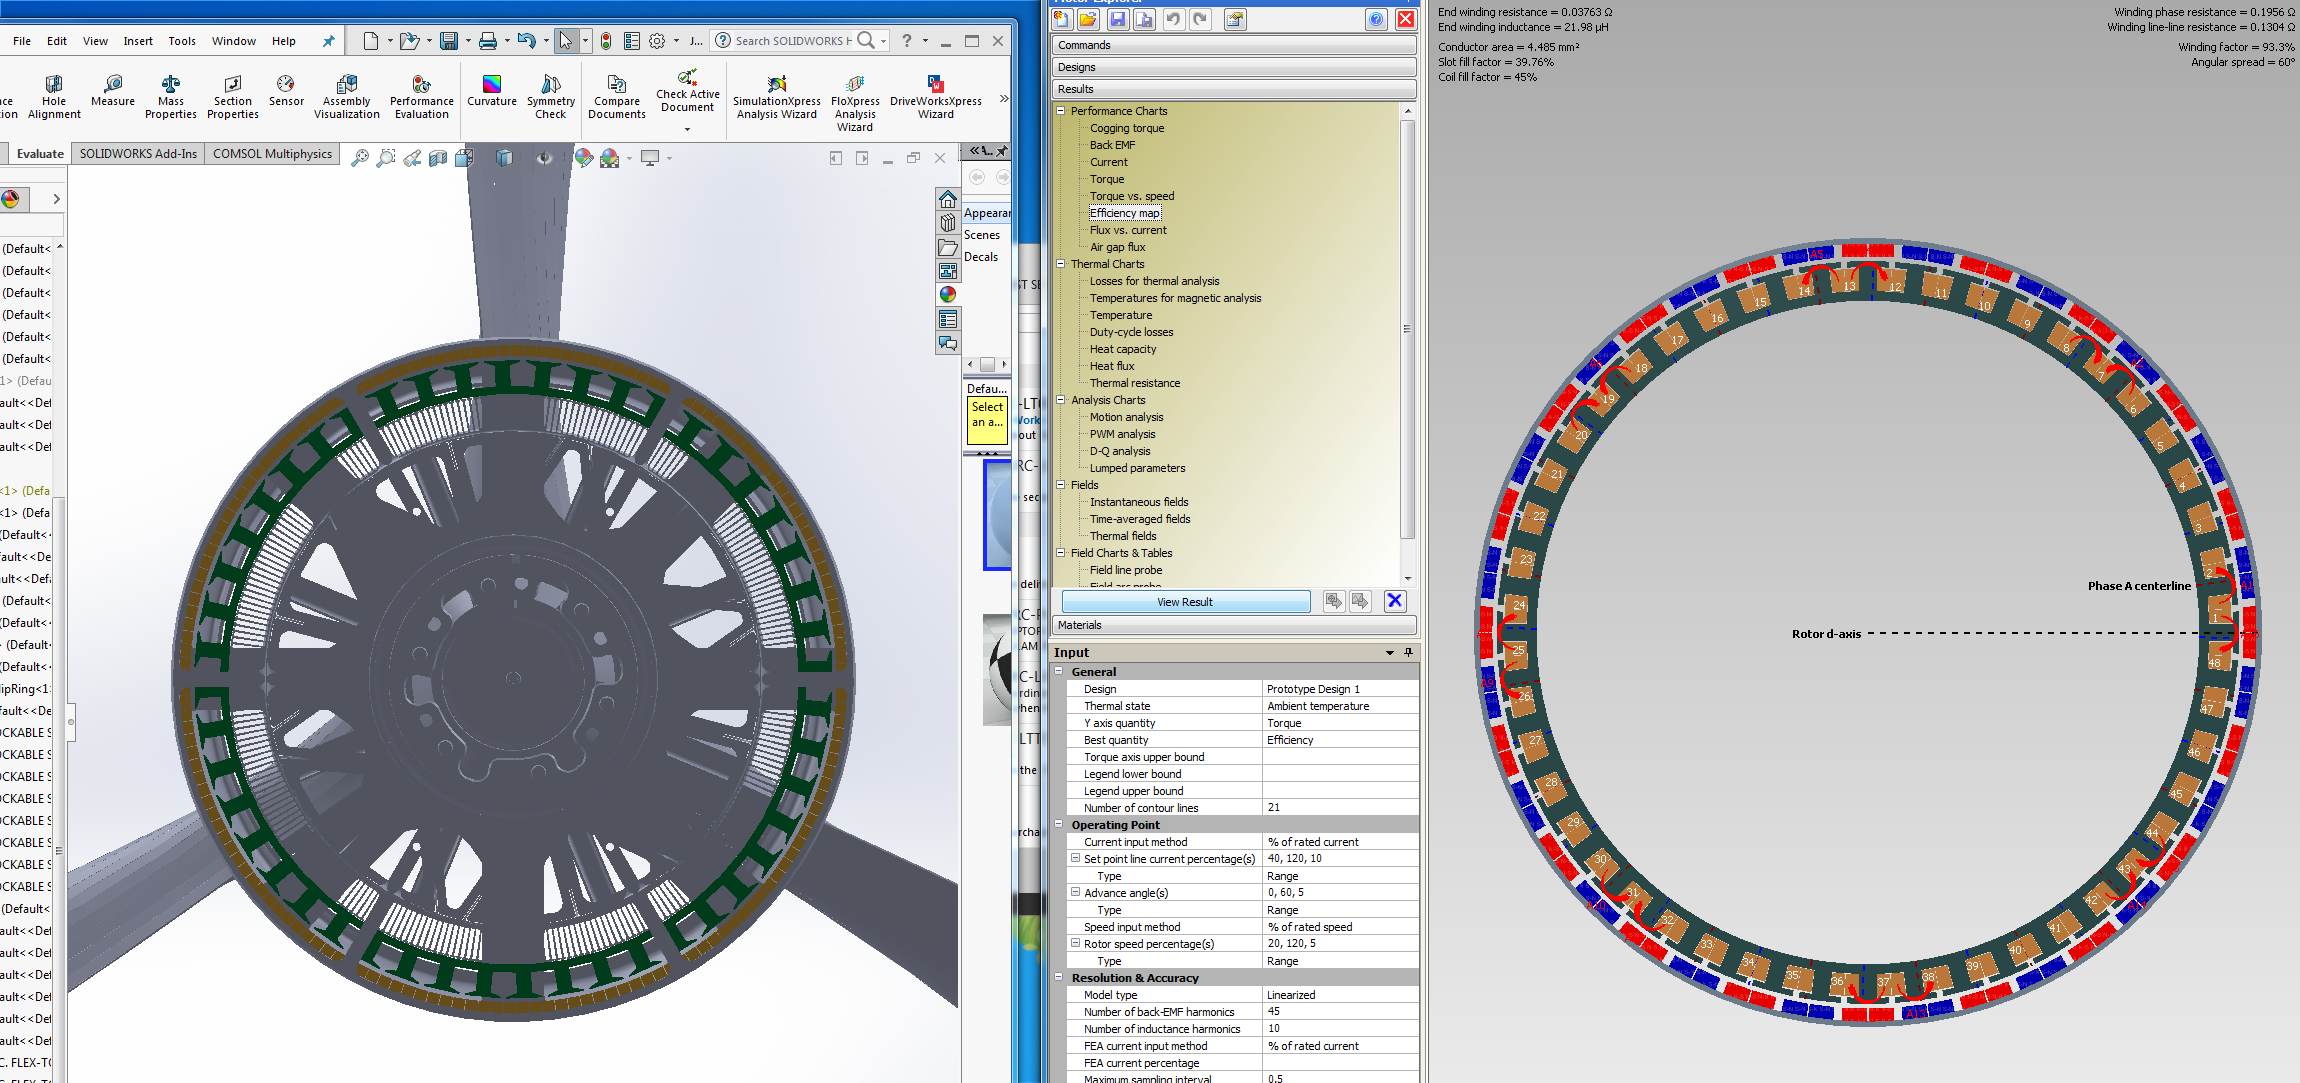
\includegraphics[width=1.0\textwidth]{figures/motorSolve.png}
	\caption{}
	\label{fig:motorSolve}
\end{figure}

\subsubsection{Stator Core Loss}
Stator core loss was predicted using the Improved Generalized Stienmetz Equation (IGSE) with minor loop separation method found in Reference \cite{CoreLoss}. The IGSE is a modification to the Stienmetz Equation that allows for accurate prediction of core loss when the magnetic field is not sinusoidal. The Stienmetz Equation defines the specific core loss (loss per Kg of material) in electrical steel subjected to a sinusoidal varying magnetic field as

\begin{equation}
P_{v} = k*f^{\alpha}B^{\beta}
\label{eq:CoreLoss}
\end{equation}

Where $P_v$ is specific core loss, f is the frequency of the sinusoidal varying magnetic field, B is the peak value of the field, 
and $k$, $\alpha$, and $\beta$ are material constants. $k$, $\alpha$, and $\beta$  
can generally be determined from core loss information provided by electrical steel manufacturers. 
Estimates of these constants for the JNEX900 laminated electrical steel used in SCEPTORs wing tip motors can be found in Table X. 
These estimates were made using charts found in Ref \cite{JFE}. The IGSE uses these parameters to predict core loss for non-sinusoidal waves as


\begin{equation}
P_{v} = \frac{1}{T}\int_{0}^{T}k_{1}|\frac{dB}{dt}|^{\alpha}(\Delta B)^{\beta-\alpha}dt
\label{eq:CoreLoss2}
\end{equation}
\begin{equation}
k_{1} = \frac{k}{2^{\beta-1}\pi^{\alpha-1}}\int_{0}^{2\pi}|cos(\theta)|^{\alpha}d\theta
\label{eq:CoreLoss2b}
\end{equation}

Where T is the period of repetition of the field in the core, $\Delta B$ is the peak to peak flux density, and $k_{1}$ is an updated loss coefficient. The algorithm for numerical implementing of this equation with minor loop separation is discussed in detail in Reference \cite{CoreLoss}. This algorithm was implemented on the magnetic field vs rotor position data from the COMSOL simulation with time normalized so that core loss at any rotational speed can be estimate by

\begin{equation}
Loss_{core} = 0.2157*f_{elec}^{\alpha}
\label{eq:CoreLoss3}
\end{equation}

Where $Loss_{core}$ is the core loss in the motor and $f_{elec}$ is the electrical frequency of the motor at a given rotational speed. At nominal motor operating conditions (2250 RPM) this predicts 966 watts of core loss. 

This loss prediction is only meant to serve as a min baseline for core loss in the motor as the IGSE most likely under predicts the core losses. The IGSE is only accurate for unidirectional fields and therefore it doesn’t account for the losses from the rotating fields in the stator tooth tips and the corners of the connection between the stator teeth and the stator back Iron \ref{Krings}. Additionally this loss estimate did not account for the effects of the pulse width modulation used to produce sinusoidal stator current. Therefore Iron Core loss is the most likely location that additionally losses need to be added based on the thermal behavior of the motor. 
\subsubsection{Eddy Currents in Magnets}
Eddy currents in the Magnets where predicted using the eddy current model for general periodic waves found in \cite{Roshen}. The model defines volumetric loss in a component experiencing a periodically varying magnetic field as 

\begin{equation}
P_{c} = \frac{d^2}{3*\pi*\rho}\frac{1}{T}\int_{0}^{T}(\frac{dB}{dt})dt
\label{eq:EddyLoss}
\end{equation}

Where $P_{c}$ is the volumetric loss, d is the thickness of the component in the direction perpendicular to the field, and $\rho$ is the resistivity of the material. This equation was applied to the magnetic field vs rotor position data with time normalized so that eddy current loss in the magnets at any rotational speed can be estimate by 
\begin{equation}
Loss_{mag} = 0.0010276*f_{elec}^{2}
\label{eq:EddyLoss2}
\end{equation}

Where $Loss_{mag}$ is the total loss in the magnets. At nominal motor operating conditions this predicts 578 watts of eddy current loss.

\subsubsection{Eddy Currents In Windings}
Eddy currents in the windings were calculated using the same equation as for the eddy currents in the magnets but with an updated coefficient so that

\begin{equation}
P_{c} = \frac{\pi a^2}{4*\rho}\frac{1}{T}\int_{0}^{T}(\frac{dB}{dt})dt
\label{eq:EddyLoss3}
\end{equation}

Where a is the wire diameter. This equation was applied to the magnetic field vs rotor position data with time normalized so that eddy current loss in the wire at any rotational speed can be estimate by

\begin{equation}
Loss_{wire,eddy} = 0.00040681*f_{elec}^{2}
\label{eq:EddyLoss4}
\end{equation}

Where $Loss_{wire,eddy}$ is the total eddy current loss in the windings. At nominal motor operating conditions this predicts 228 watts of eddy current loss.

\subsubsection{Mechanical Losses}

Mechanical losses are separated into windage and bearing losses. Windage losses are calculated in the airgap and on the axial faces of the rotor. 
The windage losses in the airgap are estimated using the model from reference \cite{Huang} where power loss is given by

\begin{equation}
P = kC_{f}\pi\rho\omega^{3}r^{4}l
\label{eq:Windage}
\end{equation}

Where P is the power loss, k is a constant equal to 2.5 for slotted surfaces, $C_{f}$ is the skin friction coefficient, $\rho$ is the density of air, $\omega$ is the rotational velocity, r is the rotor radius, and l is the axial length of the rotor. $C_{f}$ for the range of operation of the motor is given by

\begin{equation}
C_{f}= 0.515*\frac{\frac{\delta^{0.3}}{r}}{Re_{\delta}^{0.5}}
\label{eq:Cf}
\end{equation}

Where $\delta$ is the airgap length and $Re_{\delta}$ is the airgap Reynolds Number given by

\begin{equation}
Re_{\delta}=\frac{\rho\omega r \delta}{\mu}
\label{eq:Re_delta}
\end{equation}

Where $\mu$ is the dynamic viscosity of air.The windage loss on the axial faces of the rotor is approximated using the loss model for disks in free space from reference \cite{Saari}. Where P is given by 

\begin{equation}
P =0.5C_{f}\rho\omega^{3}(r_{2}^{5}-r_{1}^{5})
\label{eq:AxialWindage}
\end{equation}

where $r_{2}$ is rotor outer radius and $r_{1}$ is the rotor inner radius, with $C_{f}$ given by

\begin{equation}
C_{f}= \frac{0.146}{Re_{r}^{2}}
\label{eq:Cf2}
\end{equation}

Where $Re_{r}$ is the tip Reynolds number given by 

\begin{equation}
Re_{\delta}=\frac{\rho\omega r^{2}}{\mu}
\label{eq:Re2}
\end{equation}

Bearing loss is estimated using the equation for bearing moment found in \cite{Krings}. Bearing loss is defined by

\begin{equation}
Loss_{bearing} = M*\omega = 0.5*\mu_{f}*D*F*\omega
\label{eq:BearingLoss}
\end{equation}

Where M is the moment, D is the bearing bore diameter, F is the load the bearing is supporting, and $\mu_{f}$ is the bearing friction coefficient. For the double row angular contact bearing in the motor $\mu_{f}$ is .0024  The mechanical loss estimate at nominal operating conditions is 60watts.


\subsubsection{Resistive Losses in Windings}
In order to predict the resistive losses in the windings, first the required torque is updated by:

\begin{equation}
\tau_{req} = \tau_{shaft} + \frac{Loss_{wire,eddy} + Loss_{mag} +Loss_{core} +Loss_{mech}}{\omega}
\label{eq:TotalLoss}
\end{equation}

Where $\tau_{shaft}$ is the output torque needed,$\omega$ is the motor rotational speed in radians per second, and $\tau_{req}$ is the torque the motor has to produce to overcome the losses and produce the shaft torque. Using $\tau_{req}$ the required current can be calculated from the static torque vs current data taken from 2D FEA by

\begin{equation}
I = \frac{0.9091*\tau_{req}-22.6806}{\sqrt{2}sin(\phi)}
\label{eq:CurrentLoss}
\end{equation}

Where I is the armature supply current and $\phi$ is the phase offset of the rotor and stator.
Resistive losses are calculated by 

\begin{equation}
Loss_{resistive} =3*R_{phase}*\frac{I}{\sqrt{2}}^{2}
\label{eq:ResLoss}
\end{equation}

Where $R_{phase}$ is given by 

\begin{equation}
R_{phase} =\frac{N*l_{turn}*\rho}{n_{p}A_{wire}}
\label{eq:Rphase}
\end{equation}

Where N is the number of turns per phase, $l_{turn}$ is the length of wire in a single turn, $n_{p}$ is the number of parallel paths per phase, and $A_{wire}$ is the cross sectional area of a single wire.
At nominal operating conditions $\tau_{req}$ is 262 Nm and $Loss_{resistive}$ is 947 watts. 


\subsubsection{Motor Model Summary}
The total loss predicted by this model at nominal motor operating condition is 2781 watts. The predicted motor efficiency is 95.6\%. As noted previously this is likely to be an underestimate of the losses. It is expected that the core loss estimate will need to be updated based on the results of thermal data from motor testing. This update will in turn increase the resistive losses in the windings as the required torque will increase accordingly.

\section{Conclusions and Future Work}

Determining motor efficiency without precision input and output power measurement capabilities required higher order modeling to compensate for multiple loss sources. 
Testing at high powers on an open-air test stand also introduced additional confounding factors that were minimized through a combination of physical and operational controls.
Completion of these tests have sufficiently reduce uncertainty margins to pave the way for full vehicle integration and testing.

\begin{figure}[!htb]% order of placement preference: here, top, bottom
	\centering
    %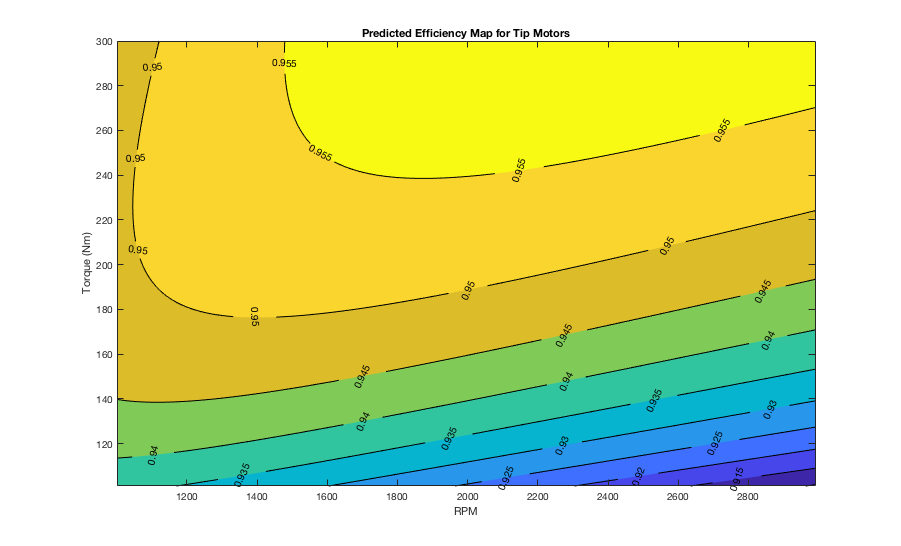
\includegraphics[width=0.5\textwidth]{figures/eff_mapNASA.png}
    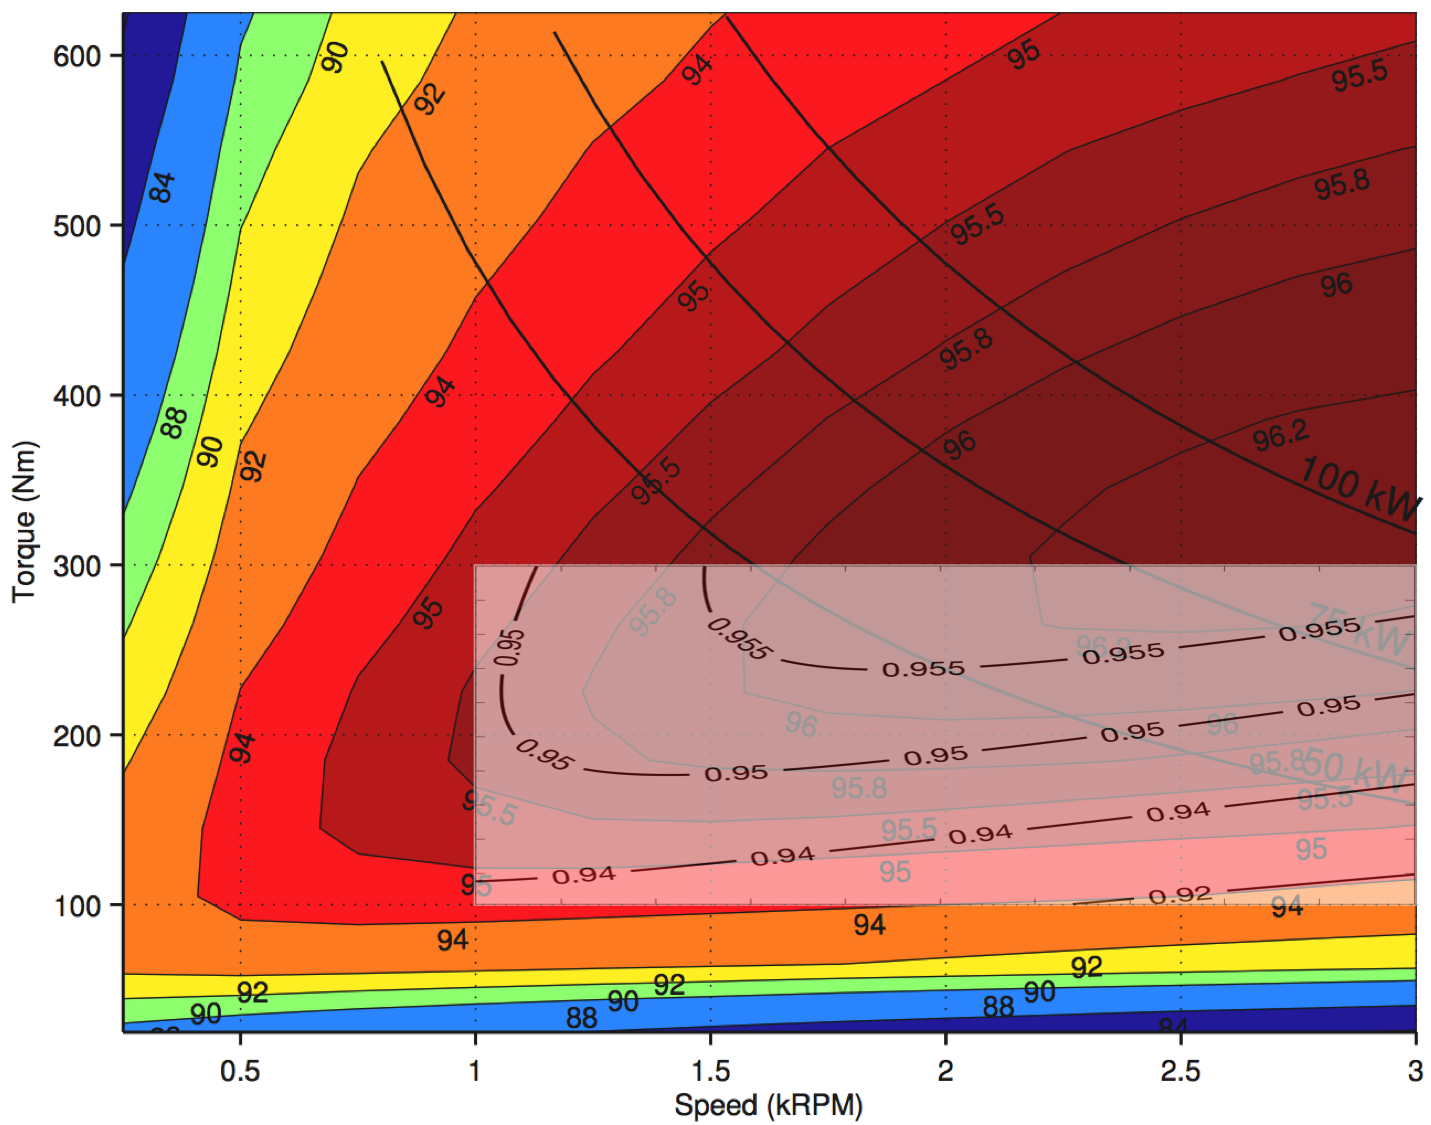
\includegraphics[width=1.0\textwidth]{figures/map_compare.png}
	\caption{Joby Efficiency Map with overlaid re-computed COMSOL Hybrid Model}
	\label{fig:map}
\end{figure}

\section{Acknowledgements}

The authors would like to thank the rest of the X-57 team, the NEAT facility, and the HEIST team for their collaboration. Scott MacAfee, from Joby motors, provided valuable and assistance about the motor manufacturing. Additional thanks to the NASA Flight Demonstration and Capabilities Project for sponsoring this work.

% produces the bibliography section when processed by BibTeX

\bibliography{bibtex_database}
\bibliographystyle{aiaa}

\end{document}

% - Release $Name:  $ -
